\documentclass[portrait, a0,30pt]{sciposter}
% Hentet fra http://iacs.epfl.ch/colloqnum06/poster.html
\usepackage[utf8]{inputenc}
\usepackage[T1]{fontenc}

\usepackage[]{wallpaper}
\usepackage[framemethod=tikz]{mdframed}
\usepackage{amsmath}
\usepackage{amssymb}
\usepackage{multicol}
\usepackage{graphicx}
\usepackage{graphicx}


\renewcommand{\sectionsize}{\Large}
\renewcommand{\authorsize}{\normalsize}
\renewcommand{\instsize}{\normalsize}

%\renewcommand{\titlesize}{\Huge}


% =========================================================
% ====== Farver og grafik øverst på siden =================
% =========================================================
% Definer farven på baggrunden i overskrifts boksene
\definecolor{BoxCol}{rgb}{0.0,0.5,0.0}
%\definecolor{BoxCol}{rgb}{0.9,0.9,1}
% baggrundsfarve for hele siden
\definecolor{mainCol}{rgb}{0.0,0.6274509803921569,0.0}

% Definer farven på tekstn i overskrifts boksene
\definecolor{SectionCol}{rgb}{1,1,1}

% Indsæt logo / billede ved siden af titlen på posteren
%\leftlogo[1.6]{fig/Trebuchet} 
\rightlogo{}
\leftlogo{}
%\leftlogo[1.5]{fig/logo.pdf} 

% Sæt bredden af de vertikale linier mellem spalterne
\setlength{\columnseprule}{0pt}
%\mdfsetup{backgroundcolor=white,roundcorner=10pt}
\mdfsetup{
innerleftmargin=1cm,innerrightmargin=1cm,roundcorner=10pt
,skipbelow=0.03cm,innerbottommargin
=1cm,innertopmargin=1cm 	
}
% Sæt afstanden mellem to kolonner
%\setlength{\columnsep}{20pt}


% =========================================================
% ====== Informationer om hvem der står bag posteren ======
% =========================================================
% Definer informationer omkring titel, forfattere og 
% organisationen bag.
\title{\fontsize{115}{5}\selectfont Visualization of Football Data}

% Note: only give author names, not institute
\author{Rasmus Bo Adeltoft, 
Sebastian Seneca Haulund Hansen, \\
Steffen Berg Klenow, 
Christian Bjørn Moeslund, \\
Andreas Staurby Olesen, 
Henrik Sejer Pedersen}
 
% insert correct institute name
\institute{Department of Mathematics and Computer Science, University of Southern Denmark}

% Kontakt adresse, kan udelades
%\email{henrik@midtiby.dk}  % shows author email address below institute

%define conference poster is presented at (appears as footer)
\conference{FF501 Poster Session, June 2016, SDU Odense}


% =========================================================
% ====== Start på selve indholdet af posteren =============
% =========================================================

\begin{document}


\CenterWallPaper{1}{fig/Football_field}

\begin{mdframed}[backgroundcolor=white,innertopmargin=2cm]

\maketitle
\end{mdframed}
%%% Begin of Multicols-Enviroment
\begin{multicols}{2}


% =========================================================
% ====== Abstract =========================================
% =========================================================



\section*{Introduction}
\begin{mdframed}
In this project, we have worked with visualization of football data. In general, visualizations can help humans’ understanding of large datasets, as the data can be summarized very effectively, and patterns can quickly be recognized.
The data at our disposal was provided by Prozone. Prozone is a company that specializes in collecting and visualizing football data.
Our visualizations were designed to compare top-tier teams with low-tier teams, and to explore how a team evolves throughout a season as well as a match.
\end{mdframed}
\section*{Visualization Design}
\begin{mdframed}
	\textbf{Marks and Channels}
	Marks are the individual elements in a graph, while channels define the appearance of these. Marks could be points in a scatterplot, and the channels could be shape or positions on common scales. 
	
	\textbf{What-why-how}
	Visualizations are made by following the what-why-how principle. \emph{What} is comprised of the semantics of the data as well as the type. \emph{Why} includes questions such as "Why make the visualization?" and "Should it consume or produce data?". \emph{How} consists of how to design the visualization, as well as how to create it.
\end{mdframed}


\begin{mdframed}[backgroundcolor=white]
	\begin{figure}[H]
		\center
		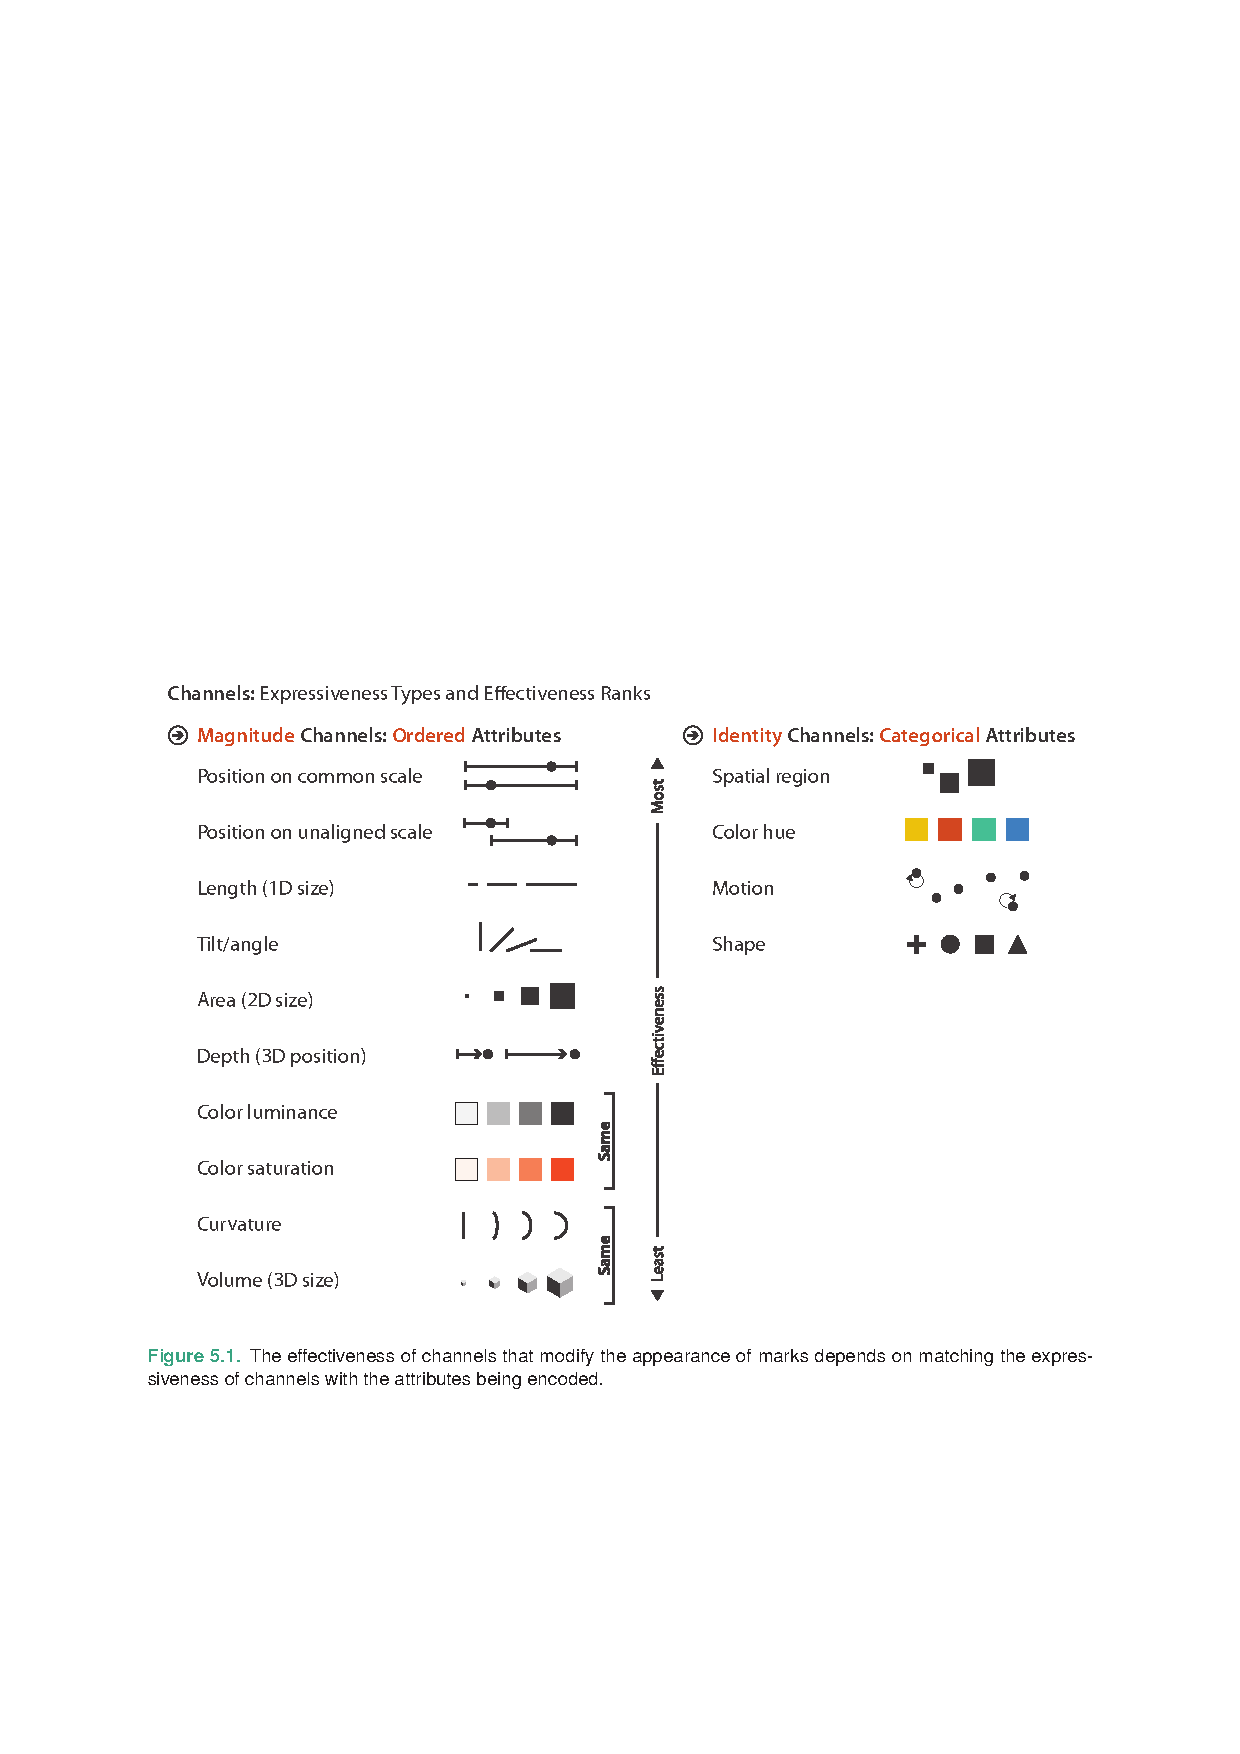
\includegraphics[width=0.9\textwidth,
		trim=80 323 75 327, clip]{fig/channels_marks_effectiveness}
		\caption{Effectiveness of different channels. 
		Source: Munzner, T. and Maguire, E. (2015) "Visualization Analysis and Design", p.115}
		\label{Fig:efficiency}
	\end{figure}
\end{mdframed}


\section*{Technology and Data}
\begin{mdframed}
To make the visualizations, we have used two kinds of technology. We have used \emph{R}, which is a programming language for statistical computing, and we have used \emph{D3}, which is a \emph{JavaScript} library for making visualizations. 

\hspace{30pt}\emph{R} is used to manipulate and clean the football data to make it ready for dynamic visualizations, but it is also used to make static ones. \emph{D3} is used to make dynamic visualizations based on the data we have cleaned in \emph{R}.
Using \emph{D3} allows us to make the visualizations interactive, and it allows users to view and interact with the visualizations in a web browser.

\hspace{30pt}The data we have used in our visualizations have been acquired through an API provided by Prozone. We have implemented access to the API directly in \emph{R}, making data acquisition and visualization generation automated.

\end{mdframed}

\section*{Conclusion}
\begin{mdframed}
With the visualizations, a few things became apparent. One of the more telling finds was that there is a tendency for teams to make more goal attempts as a match progresses. Furthermore, when a team loses to a lower ranked team, the higher ranked team fails more passes than usual, and tends to play more towards the middle of the field.
These tendencies were found on the field-based visualizations, which proved to be efficient idioms for our purpose.
\end{mdframed}
\begin{tikzpicture}[remember picture,overlay]
\node [xshift=-31cm,yshift=-17cm] at (current page.north)
{

\includegraphics[scale=1]{fig/logo}
};
\end{tikzpicture}

\begin{mdframed}
\begin{figure}
	\center
	\includegraphics[width=\textwidth,trim = 120 47 120 70, clip]{fig/"test".pdf}
	\label{Fig:viz}
	\caption{Three matches played between FCM and Viborg, plotted from FCM's point of view. The color illustrates whether FCM lost (red) or won (blue).}
\end{figure}
\end{mdframed}

\begin{mdframed}
\begin{figure}
	\center
	\includegraphics[width=\textwidth,trim = 20 618 54 142, clip]{fig/"GoalAT".pdf}
	\label{Fig:viz}
	\caption{The map shows clustering of certain events in an entire season. In this snapshot, goal attempts between 70 and 80 minutes are shown.}
\end{figure}
\end{mdframed}

\begin{mdframed}
\begin{figure}
\center
\includegraphics[width=\textwidth, trim = 0 90 0 80,clip]{fig/"Nationality of the Players".pdf}
\label{Fig:Nationality}
\caption{A Sankey-Chart showing the distribution of players' nationality in the Danish Super League.
}
\end{figure}
\end{mdframed}

%\begin{thebibliography}{m}
%
%\bibitem{areference}
%An Author
%{\em A reference}.
%A paper.

%\bibitem{somepaper}
%An Other Author
%{\em A reference}.
%Some paper.


%\end{thebibliography}



\end{multicols}

\end{document}

